
% Default to the notebook output style

    


% Inherit from the specified cell style.




    
\documentclass[11pt]{article}

    
    
    \usepackage[T1]{fontenc}
    % Nicer default font (+ math font) than Computer Modern for most use cases
    \usepackage{mathpazo}

    % Basic figure setup, for now with no caption control since it's done
    % automatically by Pandoc (which extracts ![](path) syntax from Markdown).
    \usepackage{graphicx}
    % We will generate all images so they have a width \maxwidth. This means
    % that they will get their normal width if they fit onto the page, but
    % are scaled down if they would overflow the margins.
    \makeatletter
    \def\maxwidth{\ifdim\Gin@nat@width>\linewidth\linewidth
    \else\Gin@nat@width\fi}
    \makeatother
    \let\Oldincludegraphics\includegraphics
    % Set max figure width to be 80% of text width, for now hardcoded.
    \renewcommand{\includegraphics}[1]{\Oldincludegraphics[width=.8\maxwidth]{#1}}
    % Ensure that by default, figures have no caption (until we provide a
    % proper Figure object with a Caption API and a way to capture that
    % in the conversion process - todo).
    \usepackage{caption}
    \DeclareCaptionLabelFormat{nolabel}{}
    \captionsetup{labelformat=nolabel}

    \usepackage{adjustbox} % Used to constrain images to a maximum size 
    \usepackage{xcolor} % Allow colors to be defined
    \usepackage{enumerate} % Needed for markdown enumerations to work
    \usepackage{geometry} % Used to adjust the document margins
    \usepackage{amsmath} % Equations
    \usepackage{amssymb} % Equations
    \usepackage{textcomp} % defines textquotesingle
    % Hack from http://tex.stackexchange.com/a/47451/13684:
    \AtBeginDocument{%
        \def\PYZsq{\textquotesingle}% Upright quotes in Pygmentized code
    }
    \usepackage{upquote} % Upright quotes for verbatim code
    \usepackage{eurosym} % defines \euro
    \usepackage[mathletters]{ucs} % Extended unicode (utf-8) support
    \usepackage[utf8x]{inputenc} % Allow utf-8 characters in the tex document
    \usepackage{fancyvrb} % verbatim replacement that allows latex
    \usepackage{grffile} % extends the file name processing of package graphics 
                         % to support a larger range 
    % The hyperref package gives us a pdf with properly built
    % internal navigation ('pdf bookmarks' for the table of contents,
    % internal cross-reference links, web links for URLs, etc.)
    \usepackage{hyperref}
    \usepackage{longtable} % longtable support required by pandoc >1.10
    \usepackage{booktabs}  % table support for pandoc > 1.12.2
    \usepackage[inline]{enumitem} % IRkernel/repr support (it uses the enumerate* environment)
    \usepackage[normalem]{ulem} % ulem is needed to support strikethroughs (\sout)
                                % normalem makes italics be italics, not underlines
    

    
    
    % Colors for the hyperref package
    \definecolor{urlcolor}{rgb}{0,.145,.698}
    \definecolor{linkcolor}{rgb}{.71,0.21,0.01}
    \definecolor{citecolor}{rgb}{.12,.54,.11}

    % ANSI colors
    \definecolor{ansi-black}{HTML}{3E424D}
    \definecolor{ansi-black-intense}{HTML}{282C36}
    \definecolor{ansi-red}{HTML}{E75C58}
    \definecolor{ansi-red-intense}{HTML}{B22B31}
    \definecolor{ansi-green}{HTML}{00A250}
    \definecolor{ansi-green-intense}{HTML}{007427}
    \definecolor{ansi-yellow}{HTML}{DDB62B}
    \definecolor{ansi-yellow-intense}{HTML}{B27D12}
    \definecolor{ansi-blue}{HTML}{208FFB}
    \definecolor{ansi-blue-intense}{HTML}{0065CA}
    \definecolor{ansi-magenta}{HTML}{D160C4}
    \definecolor{ansi-magenta-intense}{HTML}{A03196}
    \definecolor{ansi-cyan}{HTML}{60C6C8}
    \definecolor{ansi-cyan-intense}{HTML}{258F8F}
    \definecolor{ansi-white}{HTML}{C5C1B4}
    \definecolor{ansi-white-intense}{HTML}{A1A6B2}

    % commands and environments needed by pandoc snippets
    % extracted from the output of `pandoc -s`
    \providecommand{\tightlist}{%
      \setlength{\itemsep}{0pt}\setlength{\parskip}{0pt}}
    \DefineVerbatimEnvironment{Highlighting}{Verbatim}{commandchars=\\\{\}}
    % Add ',fontsize=\small' for more characters per line
    \newenvironment{Shaded}{}{}
    \newcommand{\KeywordTok}[1]{\textcolor[rgb]{0.00,0.44,0.13}{\textbf{{#1}}}}
    \newcommand{\DataTypeTok}[1]{\textcolor[rgb]{0.56,0.13,0.00}{{#1}}}
    \newcommand{\DecValTok}[1]{\textcolor[rgb]{0.25,0.63,0.44}{{#1}}}
    \newcommand{\BaseNTok}[1]{\textcolor[rgb]{0.25,0.63,0.44}{{#1}}}
    \newcommand{\FloatTok}[1]{\textcolor[rgb]{0.25,0.63,0.44}{{#1}}}
    \newcommand{\CharTok}[1]{\textcolor[rgb]{0.25,0.44,0.63}{{#1}}}
    \newcommand{\StringTok}[1]{\textcolor[rgb]{0.25,0.44,0.63}{{#1}}}
    \newcommand{\CommentTok}[1]{\textcolor[rgb]{0.38,0.63,0.69}{\textit{{#1}}}}
    \newcommand{\OtherTok}[1]{\textcolor[rgb]{0.00,0.44,0.13}{{#1}}}
    \newcommand{\AlertTok}[1]{\textcolor[rgb]{1.00,0.00,0.00}{\textbf{{#1}}}}
    \newcommand{\FunctionTok}[1]{\textcolor[rgb]{0.02,0.16,0.49}{{#1}}}
    \newcommand{\RegionMarkerTok}[1]{{#1}}
    \newcommand{\ErrorTok}[1]{\textcolor[rgb]{1.00,0.00,0.00}{\textbf{{#1}}}}
    \newcommand{\NormalTok}[1]{{#1}}
    
    % Additional commands for more recent versions of Pandoc
    \newcommand{\ConstantTok}[1]{\textcolor[rgb]{0.53,0.00,0.00}{{#1}}}
    \newcommand{\SpecialCharTok}[1]{\textcolor[rgb]{0.25,0.44,0.63}{{#1}}}
    \newcommand{\VerbatimStringTok}[1]{\textcolor[rgb]{0.25,0.44,0.63}{{#1}}}
    \newcommand{\SpecialStringTok}[1]{\textcolor[rgb]{0.73,0.40,0.53}{{#1}}}
    \newcommand{\ImportTok}[1]{{#1}}
    \newcommand{\DocumentationTok}[1]{\textcolor[rgb]{0.73,0.13,0.13}{\textit{{#1}}}}
    \newcommand{\AnnotationTok}[1]{\textcolor[rgb]{0.38,0.63,0.69}{\textbf{\textit{{#1}}}}}
    \newcommand{\CommentVarTok}[1]{\textcolor[rgb]{0.38,0.63,0.69}{\textbf{\textit{{#1}}}}}
    \newcommand{\VariableTok}[1]{\textcolor[rgb]{0.10,0.09,0.49}{{#1}}}
    \newcommand{\ControlFlowTok}[1]{\textcolor[rgb]{0.00,0.44,0.13}{\textbf{{#1}}}}
    \newcommand{\OperatorTok}[1]{\textcolor[rgb]{0.40,0.40,0.40}{{#1}}}
    \newcommand{\BuiltInTok}[1]{{#1}}
    \newcommand{\ExtensionTok}[1]{{#1}}
    \newcommand{\PreprocessorTok}[1]{\textcolor[rgb]{0.74,0.48,0.00}{{#1}}}
    \newcommand{\AttributeTok}[1]{\textcolor[rgb]{0.49,0.56,0.16}{{#1}}}
    \newcommand{\InformationTok}[1]{\textcolor[rgb]{0.38,0.63,0.69}{\textbf{\textit{{#1}}}}}
    \newcommand{\WarningTok}[1]{\textcolor[rgb]{0.38,0.63,0.69}{\textbf{\textit{{#1}}}}}
    
    
    % Define a nice break command that doesn't care if a line doesn't already
    % exist.
    \def\br{\hspace*{\fill} \\* }
    % Math Jax compatability definitions
    \def\gt{>}
    \def\lt{<}
    % Document parameters
    \title{DIP-HW6}
    
    
    

    % Pygments definitions
    
\makeatletter
\def\PY@reset{\let\PY@it=\relax \let\PY@bf=\relax%
    \let\PY@ul=\relax \let\PY@tc=\relax%
    \let\PY@bc=\relax \let\PY@ff=\relax}
\def\PY@tok#1{\csname PY@tok@#1\endcsname}
\def\PY@toks#1+{\ifx\relax#1\empty\else%
    \PY@tok{#1}\expandafter\PY@toks\fi}
\def\PY@do#1{\PY@bc{\PY@tc{\PY@ul{%
    \PY@it{\PY@bf{\PY@ff{#1}}}}}}}
\def\PY#1#2{\PY@reset\PY@toks#1+\relax+\PY@do{#2}}

\expandafter\def\csname PY@tok@w\endcsname{\def\PY@tc##1{\textcolor[rgb]{0.73,0.73,0.73}{##1}}}
\expandafter\def\csname PY@tok@c\endcsname{\let\PY@it=\textit\def\PY@tc##1{\textcolor[rgb]{0.25,0.50,0.50}{##1}}}
\expandafter\def\csname PY@tok@cp\endcsname{\def\PY@tc##1{\textcolor[rgb]{0.74,0.48,0.00}{##1}}}
\expandafter\def\csname PY@tok@k\endcsname{\let\PY@bf=\textbf\def\PY@tc##1{\textcolor[rgb]{0.00,0.50,0.00}{##1}}}
\expandafter\def\csname PY@tok@kp\endcsname{\def\PY@tc##1{\textcolor[rgb]{0.00,0.50,0.00}{##1}}}
\expandafter\def\csname PY@tok@kt\endcsname{\def\PY@tc##1{\textcolor[rgb]{0.69,0.00,0.25}{##1}}}
\expandafter\def\csname PY@tok@o\endcsname{\def\PY@tc##1{\textcolor[rgb]{0.40,0.40,0.40}{##1}}}
\expandafter\def\csname PY@tok@ow\endcsname{\let\PY@bf=\textbf\def\PY@tc##1{\textcolor[rgb]{0.67,0.13,1.00}{##1}}}
\expandafter\def\csname PY@tok@nb\endcsname{\def\PY@tc##1{\textcolor[rgb]{0.00,0.50,0.00}{##1}}}
\expandafter\def\csname PY@tok@nf\endcsname{\def\PY@tc##1{\textcolor[rgb]{0.00,0.00,1.00}{##1}}}
\expandafter\def\csname PY@tok@nc\endcsname{\let\PY@bf=\textbf\def\PY@tc##1{\textcolor[rgb]{0.00,0.00,1.00}{##1}}}
\expandafter\def\csname PY@tok@nn\endcsname{\let\PY@bf=\textbf\def\PY@tc##1{\textcolor[rgb]{0.00,0.00,1.00}{##1}}}
\expandafter\def\csname PY@tok@ne\endcsname{\let\PY@bf=\textbf\def\PY@tc##1{\textcolor[rgb]{0.82,0.25,0.23}{##1}}}
\expandafter\def\csname PY@tok@nv\endcsname{\def\PY@tc##1{\textcolor[rgb]{0.10,0.09,0.49}{##1}}}
\expandafter\def\csname PY@tok@no\endcsname{\def\PY@tc##1{\textcolor[rgb]{0.53,0.00,0.00}{##1}}}
\expandafter\def\csname PY@tok@nl\endcsname{\def\PY@tc##1{\textcolor[rgb]{0.63,0.63,0.00}{##1}}}
\expandafter\def\csname PY@tok@ni\endcsname{\let\PY@bf=\textbf\def\PY@tc##1{\textcolor[rgb]{0.60,0.60,0.60}{##1}}}
\expandafter\def\csname PY@tok@na\endcsname{\def\PY@tc##1{\textcolor[rgb]{0.49,0.56,0.16}{##1}}}
\expandafter\def\csname PY@tok@nt\endcsname{\let\PY@bf=\textbf\def\PY@tc##1{\textcolor[rgb]{0.00,0.50,0.00}{##1}}}
\expandafter\def\csname PY@tok@nd\endcsname{\def\PY@tc##1{\textcolor[rgb]{0.67,0.13,1.00}{##1}}}
\expandafter\def\csname PY@tok@s\endcsname{\def\PY@tc##1{\textcolor[rgb]{0.73,0.13,0.13}{##1}}}
\expandafter\def\csname PY@tok@sd\endcsname{\let\PY@it=\textit\def\PY@tc##1{\textcolor[rgb]{0.73,0.13,0.13}{##1}}}
\expandafter\def\csname PY@tok@si\endcsname{\let\PY@bf=\textbf\def\PY@tc##1{\textcolor[rgb]{0.73,0.40,0.53}{##1}}}
\expandafter\def\csname PY@tok@se\endcsname{\let\PY@bf=\textbf\def\PY@tc##1{\textcolor[rgb]{0.73,0.40,0.13}{##1}}}
\expandafter\def\csname PY@tok@sr\endcsname{\def\PY@tc##1{\textcolor[rgb]{0.73,0.40,0.53}{##1}}}
\expandafter\def\csname PY@tok@ss\endcsname{\def\PY@tc##1{\textcolor[rgb]{0.10,0.09,0.49}{##1}}}
\expandafter\def\csname PY@tok@sx\endcsname{\def\PY@tc##1{\textcolor[rgb]{0.00,0.50,0.00}{##1}}}
\expandafter\def\csname PY@tok@m\endcsname{\def\PY@tc##1{\textcolor[rgb]{0.40,0.40,0.40}{##1}}}
\expandafter\def\csname PY@tok@gh\endcsname{\let\PY@bf=\textbf\def\PY@tc##1{\textcolor[rgb]{0.00,0.00,0.50}{##1}}}
\expandafter\def\csname PY@tok@gu\endcsname{\let\PY@bf=\textbf\def\PY@tc##1{\textcolor[rgb]{0.50,0.00,0.50}{##1}}}
\expandafter\def\csname PY@tok@gd\endcsname{\def\PY@tc##1{\textcolor[rgb]{0.63,0.00,0.00}{##1}}}
\expandafter\def\csname PY@tok@gi\endcsname{\def\PY@tc##1{\textcolor[rgb]{0.00,0.63,0.00}{##1}}}
\expandafter\def\csname PY@tok@gr\endcsname{\def\PY@tc##1{\textcolor[rgb]{1.00,0.00,0.00}{##1}}}
\expandafter\def\csname PY@tok@ge\endcsname{\let\PY@it=\textit}
\expandafter\def\csname PY@tok@gs\endcsname{\let\PY@bf=\textbf}
\expandafter\def\csname PY@tok@gp\endcsname{\let\PY@bf=\textbf\def\PY@tc##1{\textcolor[rgb]{0.00,0.00,0.50}{##1}}}
\expandafter\def\csname PY@tok@go\endcsname{\def\PY@tc##1{\textcolor[rgb]{0.53,0.53,0.53}{##1}}}
\expandafter\def\csname PY@tok@gt\endcsname{\def\PY@tc##1{\textcolor[rgb]{0.00,0.27,0.87}{##1}}}
\expandafter\def\csname PY@tok@err\endcsname{\def\PY@bc##1{\setlength{\fboxsep}{0pt}\fcolorbox[rgb]{1.00,0.00,0.00}{1,1,1}{\strut ##1}}}
\expandafter\def\csname PY@tok@kc\endcsname{\let\PY@bf=\textbf\def\PY@tc##1{\textcolor[rgb]{0.00,0.50,0.00}{##1}}}
\expandafter\def\csname PY@tok@kd\endcsname{\let\PY@bf=\textbf\def\PY@tc##1{\textcolor[rgb]{0.00,0.50,0.00}{##1}}}
\expandafter\def\csname PY@tok@kn\endcsname{\let\PY@bf=\textbf\def\PY@tc##1{\textcolor[rgb]{0.00,0.50,0.00}{##1}}}
\expandafter\def\csname PY@tok@kr\endcsname{\let\PY@bf=\textbf\def\PY@tc##1{\textcolor[rgb]{0.00,0.50,0.00}{##1}}}
\expandafter\def\csname PY@tok@bp\endcsname{\def\PY@tc##1{\textcolor[rgb]{0.00,0.50,0.00}{##1}}}
\expandafter\def\csname PY@tok@fm\endcsname{\def\PY@tc##1{\textcolor[rgb]{0.00,0.00,1.00}{##1}}}
\expandafter\def\csname PY@tok@vc\endcsname{\def\PY@tc##1{\textcolor[rgb]{0.10,0.09,0.49}{##1}}}
\expandafter\def\csname PY@tok@vg\endcsname{\def\PY@tc##1{\textcolor[rgb]{0.10,0.09,0.49}{##1}}}
\expandafter\def\csname PY@tok@vi\endcsname{\def\PY@tc##1{\textcolor[rgb]{0.10,0.09,0.49}{##1}}}
\expandafter\def\csname PY@tok@vm\endcsname{\def\PY@tc##1{\textcolor[rgb]{0.10,0.09,0.49}{##1}}}
\expandafter\def\csname PY@tok@sa\endcsname{\def\PY@tc##1{\textcolor[rgb]{0.73,0.13,0.13}{##1}}}
\expandafter\def\csname PY@tok@sb\endcsname{\def\PY@tc##1{\textcolor[rgb]{0.73,0.13,0.13}{##1}}}
\expandafter\def\csname PY@tok@sc\endcsname{\def\PY@tc##1{\textcolor[rgb]{0.73,0.13,0.13}{##1}}}
\expandafter\def\csname PY@tok@dl\endcsname{\def\PY@tc##1{\textcolor[rgb]{0.73,0.13,0.13}{##1}}}
\expandafter\def\csname PY@tok@s2\endcsname{\def\PY@tc##1{\textcolor[rgb]{0.73,0.13,0.13}{##1}}}
\expandafter\def\csname PY@tok@sh\endcsname{\def\PY@tc##1{\textcolor[rgb]{0.73,0.13,0.13}{##1}}}
\expandafter\def\csname PY@tok@s1\endcsname{\def\PY@tc##1{\textcolor[rgb]{0.73,0.13,0.13}{##1}}}
\expandafter\def\csname PY@tok@mb\endcsname{\def\PY@tc##1{\textcolor[rgb]{0.40,0.40,0.40}{##1}}}
\expandafter\def\csname PY@tok@mf\endcsname{\def\PY@tc##1{\textcolor[rgb]{0.40,0.40,0.40}{##1}}}
\expandafter\def\csname PY@tok@mh\endcsname{\def\PY@tc##1{\textcolor[rgb]{0.40,0.40,0.40}{##1}}}
\expandafter\def\csname PY@tok@mi\endcsname{\def\PY@tc##1{\textcolor[rgb]{0.40,0.40,0.40}{##1}}}
\expandafter\def\csname PY@tok@il\endcsname{\def\PY@tc##1{\textcolor[rgb]{0.40,0.40,0.40}{##1}}}
\expandafter\def\csname PY@tok@mo\endcsname{\def\PY@tc##1{\textcolor[rgb]{0.40,0.40,0.40}{##1}}}
\expandafter\def\csname PY@tok@ch\endcsname{\let\PY@it=\textit\def\PY@tc##1{\textcolor[rgb]{0.25,0.50,0.50}{##1}}}
\expandafter\def\csname PY@tok@cm\endcsname{\let\PY@it=\textit\def\PY@tc##1{\textcolor[rgb]{0.25,0.50,0.50}{##1}}}
\expandafter\def\csname PY@tok@cpf\endcsname{\let\PY@it=\textit\def\PY@tc##1{\textcolor[rgb]{0.25,0.50,0.50}{##1}}}
\expandafter\def\csname PY@tok@c1\endcsname{\let\PY@it=\textit\def\PY@tc##1{\textcolor[rgb]{0.25,0.50,0.50}{##1}}}
\expandafter\def\csname PY@tok@cs\endcsname{\let\PY@it=\textit\def\PY@tc##1{\textcolor[rgb]{0.25,0.50,0.50}{##1}}}

\def\PYZbs{\char`\\}
\def\PYZus{\char`\_}
\def\PYZob{\char`\{}
\def\PYZcb{\char`\}}
\def\PYZca{\char`\^}
\def\PYZam{\char`\&}
\def\PYZlt{\char`\<}
\def\PYZgt{\char`\>}
\def\PYZsh{\char`\#}
\def\PYZpc{\char`\%}
\def\PYZdl{\char`\$}
\def\PYZhy{\char`\-}
\def\PYZsq{\char`\'}
\def\PYZdq{\char`\"}
\def\PYZti{\char`\~}
% for compatibility with earlier versions
\def\PYZat{@}
\def\PYZlb{[}
\def\PYZrb{]}
\makeatother


    % Exact colors from NB
    \definecolor{incolor}{rgb}{0.0, 0.0, 0.5}
    \definecolor{outcolor}{rgb}{0.545, 0.0, 0.0}



    
    % Prevent overflowing lines due to hard-to-break entities
    \sloppy 
    % Setup hyperref package
    \hypersetup{
      breaklinks=true,  % so long urls are correctly broken across lines
      colorlinks=true,
      urlcolor=urlcolor,
      linkcolor=linkcolor,
      citecolor=citecolor,
      }
    % Slightly bigger margins than the latex defaults
    
    \geometry{verbose,tmargin=1in,bmargin=1in,lmargin=1in,rmargin=1in}
    
    

    \begin{document}
    
    
    \maketitle
    
    

    
    \hypertarget{digital-image-processing---hw6---98722278---mohammad-doosti-lakhani}{%
\section{Digital Image Processing - HW6 - 98722278 - Mohammad Doosti
Lakhani}\label{digital-image-processing---hw6---98722278---mohammad-doosti-lakhani}}

In this notebook, I have solved the assignment's problems which are as
follows:

\begin{enumerate}
\def\labelenumi{\arabic{enumi}.}
\tightlist
\item
  This step consists of following tasks:

  \begin{enumerate}
  \def\labelenumii{\arabic{enumii}.}
  \tightlist
  \item
    Read
    \href{http://cseweb.ucsd.edu/~mdailey/Face-Coord/ellipse-specific-fitting.pdf}{This
    paper} and summarize it
  \item
    Convert MATLAB code in fig. 7 to python and extract ellipse
    parameters of \texttt{circle.bmp} and \texttt{ellipse.bmp} images.
  \item
    Plot estimated ellipses using \texttt{cv2.ellipse()} method.
  \end{enumerate}
\item
  We want to find the parameters of ellipse using RANSAC algorithm. If
  only \%40 of edges in the image belong to ellipse's edges and we want
  to obtain the correct parameters with probability of 0.999, how many
  iterations are required?
\item
  Do these steps in this task:

  \begin{enumerate}
  \def\labelenumii{\arabic{enumii}.}
  \tightlist
  \item
    Estimates parameters of ellipse using code in task 1 on
    \texttt{ellipse\_noise.bmp} image
  \item
    As there are points that do not blong to ellipse, RANSAC is better
    solution here. Implement RANSAC
  \item
    Draw the output on \texttt{ellipse\_noise.bmp} image
  \item
    Set the probability of achieving correct parameters of ellipse to
    0.99 and run algorithm for 10000 times. In how many of iterations,
    the estimated parameters are correct?
  \item
    Analyze your answer
  \end{enumerate}
\end{enumerate}

    \hypertarget{this-step-consists-of-following-tasks}{%
\subsection{1 This step consists of following
tasks:}\label{this-step-consists-of-following-tasks}}

\begin{enumerate}
\def\labelenumi{\arabic{enumi}.}
\tightlist
\item
  Read This paper and summarize it
\item
  Convert MATLAB code in fig. 7 to python and extract ellipse parameters
  of circle.bmp and ellipse.bmp images.
\item
  Plot estimated ellipses using cv2.ellipse() method.
\end{enumerate}

    \hypertarget{a-paper-summarization}{%
\subsubsection{1.A Paper Summarization}\label{a-paper-summarization}}

The proposed method is ellipse specified which means no matter given
data, a ellipse will be output. On top of that, it is computationally
cheap and robust to noises. The major reason that this approach is
robust and fast is that it uses least-square transformation.

First of all, they use a distance matrix with respect to ellipse
equation which is called \emph{distance\_matrix}:

Ellipse Equation: 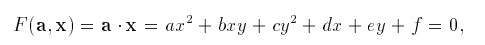
\includegraphics{wiki/eq.jpg}

Distance Matrix: 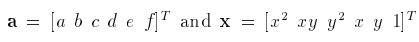
\includegraphics{wiki/dm.jpg}

Now, the parameter \texttt{a} is constrained using matrix called
\texttt{C} which is 6x6 and all these constraints are linear or
\texttt{C.dot(a)\ =\ 1}. But in this paper, constrained \texttt{a} is in
the way that forces the fitted model to be ellipse.
\texttt{4*a*c-b**2\ =\ 1} is the equality constraint where
\texttt{a.T.dot(C).dot(a)\ =\ 1}.

So \texttt{C} is:

\begin{figure}
\centering
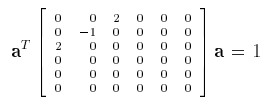
\includegraphics{wiki/c.jpg}
\caption{constraint matrix}
\end{figure}

Based on what they have covered so far, the solution of the
quadratically constrained minimization will be:

\begin{figure}
\centering

\includegraphics{wiki/cm.jpg}
\caption{constraint minimization}
\end{figure}

Furthermore, this system can be written as below image where
\texttt{lambda} is Lagrange multiplier and \texttt{S} is
\texttt{D.T.dot(D)}:

\begin{figure}
\centering
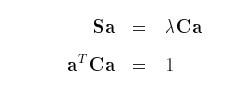
\includegraphics{wiki/ss.jpg}
\caption{simplified eigen system}
\end{figure}

This system can be solved using generalized eigenvectors of
\texttt{S.dot(a)\ =\ lambda*C.dot(a)}. In the end, if
\texttt{(lambda,\ u)} solves \texttt{S.dot(a)\ =\ lambda*C.dot(a)}, we
have:

\begin{figure}
\centering
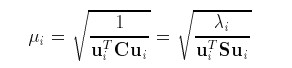
\includegraphics{wiki/mu.jpg}
\caption{mu}
\end{figure}

Then \texttt{a} can be obtained by \texttt{a\ =\ mu*u}.

    \hypertarget{b-direct-least-square-of-fitting-ellipse-implementation-and-ellipse-of-circle.bmp-and-ellipse.bmp}{%
\subsubsection{\texorpdfstring{1.B Direct Least Square of Fitting
Ellipse Implementation and Ellipse of \texttt{circle.bmp} and
\texttt{ellipse.bmp}}{1.B Direct Least Square of Fitting Ellipse Implementation and Ellipse of circle.bmp and ellipse.bmp}}\label{b-direct-least-square-of-fitting-ellipse-implementation-and-ellipse-of-circle.bmp-and-ellipse.bmp}}

    \begin{Verbatim}[commandchars=\\\{\}]
{\color{incolor}In [{\color{incolor}4}]:} \PY{k+kn}{import} \PY{n+nn}{numpy} \PY{k}{as} \PY{n+nn}{np}
        \PY{k+kn}{import} \PY{n+nn}{matplotlib}\PY{n+nn}{.}\PY{n+nn}{pyplot} \PY{k}{as} \PY{n+nn}{plt}
        \PY{k+kn}{import} \PY{n+nn}{cv2}
        \PY{o}{\PYZpc{}}\PY{k}{matplotlib} inline
\end{Verbatim}


    \begin{Verbatim}[commandchars=\\\{\}]
{\color{incolor}In [{\color{incolor}184}]:} \PY{k}{def} \PY{n+nf}{direct\PYZus{}least\PYZus{}square}\PY{p}{(}\PY{n}{x}\PY{p}{,} \PY{n}{y}\PY{p}{)}\PY{p}{:}
              \PY{n}{D} \PY{o}{=} \PY{n}{np}\PY{o}{.}\PY{n}{mat}\PY{p}{(}\PY{n}{np}\PY{o}{.}\PY{n}{vstack}\PY{p}{(}\PY{p}{[}\PY{n}{x}\PY{o}{*}\PY{o}{*}\PY{l+m+mi}{2}\PY{p}{,} \PY{n}{x}\PY{o}{*}\PY{n}{y}\PY{p}{,} \PY{n}{y}\PY{o}{*}\PY{o}{*}\PY{l+m+mi}{2}\PY{p}{,} \PY{n}{x}\PY{p}{,} \PY{n}{y}\PY{p}{,} \PY{n}{np}\PY{o}{.}\PY{n}{ones}\PY{p}{(}\PY{n+nb}{len}\PY{p}{(}\PY{n}{x}\PY{p}{)}\PY{p}{)}\PY{p}{]}\PY{p}{)}\PY{p}{)}\PY{o}{.}\PY{n}{T}
              \PY{n}{S} \PY{o}{=} \PY{n}{np}\PY{o}{.}\PY{n}{dot}\PY{p}{(}\PY{n}{D}\PY{o}{.}\PY{n}{T}\PY{p}{,} \PY{n}{D}\PY{p}{)}
              \PY{n}{C} \PY{o}{=} \PY{n}{np}\PY{o}{.}\PY{n}{zeros}\PY{p}{(}\PY{p}{(}\PY{l+m+mi}{6}\PY{p}{,} \PY{l+m+mi}{6}\PY{p}{)}\PY{p}{)}
              \PY{n}{C}\PY{p}{[}\PY{l+m+mi}{0}\PY{p}{,} \PY{l+m+mi}{2}\PY{p}{]} \PY{o}{=} \PY{l+m+mi}{2}
              \PY{n}{C}\PY{p}{[}\PY{l+m+mi}{1}\PY{p}{,} \PY{l+m+mi}{1}\PY{p}{]} \PY{o}{=} \PY{o}{\PYZhy{}}\PY{l+m+mi}{1}
              \PY{n}{C}\PY{p}{[}\PY{l+m+mi}{2}\PY{p}{,} \PY{l+m+mi}{0}\PY{p}{]} \PY{o}{=} \PY{l+m+mi}{2}
              \PY{n}{Z} \PY{o}{=} \PY{n}{np}\PY{o}{.}\PY{n}{dot}\PY{p}{(}\PY{n}{np}\PY{o}{.}\PY{n}{linalg}\PY{o}{.}\PY{n}{inv}\PY{p}{(}\PY{n}{S}\PY{p}{)}\PY{p}{,} \PY{n}{C}\PY{p}{)}
              \PY{n}{eigen\PYZus{}value}\PY{p}{,} \PY{n}{eigen\PYZus{}vec} \PY{o}{=} \PY{n}{np}\PY{o}{.}\PY{n}{linalg}\PY{o}{.}\PY{n}{eig}\PY{p}{(}\PY{n}{Z}\PY{p}{)}
              \PY{n}{eigen\PYZus{}value} \PY{o}{=} \PY{n}{eigen\PYZus{}value}\PY{o}{.}\PY{n}{reshape}\PY{p}{(}\PY{l+m+mi}{1}\PY{p}{,} \PY{o}{\PYZhy{}}\PY{l+m+mi}{1}\PY{p}{)}
              \PY{n}{pos\PYZus{}r}\PY{p}{,} \PY{n}{pos\PYZus{}c} \PY{o}{=} \PY{n}{np}\PY{o}{.}\PY{n}{where}\PY{p}{(}\PY{n}{eigen\PYZus{}value}\PY{o}{\PYZgt{}}\PY{l+m+mi}{0} \PY{o}{\PYZam{}} \PY{o}{\PYZti{}}\PY{n}{np}\PY{o}{.}\PY{n}{isinf}\PY{p}{(}\PY{n}{eigen\PYZus{}value}\PY{p}{)}\PY{p}{)}
              \PY{n}{a} \PY{o}{=} \PY{n}{eigen\PYZus{}vec}\PY{p}{[}\PY{p}{:}\PY{p}{,} \PY{n}{pos\PYZus{}c}\PY{p}{]}
              \PY{k}{return} \PY{n}{a}
          
          \PY{k}{def} \PY{n+nf}{ellipse\PYZus{}center}\PY{p}{(}\PY{n}{a}\PY{p}{)}\PY{p}{:}
              \PY{n}{a} \PY{o}{=} \PY{n}{a}\PY{o}{.}\PY{n}{reshape}\PY{p}{(}\PY{o}{\PYZhy{}}\PY{l+m+mi}{1}\PY{p}{,} \PY{l+m+mi}{1}\PY{p}{)}
              \PY{n}{b}\PY{p}{,}\PY{n}{c}\PY{p}{,}\PY{n}{d}\PY{p}{,}\PY{n}{f}\PY{p}{,}\PY{n}{g}\PY{p}{,}\PY{n}{a} \PY{o}{=} \PY{n}{a}\PY{p}{[}\PY{l+m+mi}{1}\PY{p}{]}\PY{o}{/}\PY{l+m+mi}{2}\PY{p}{,} \PY{n}{a}\PY{p}{[}\PY{l+m+mi}{2}\PY{p}{]}\PY{p}{,} \PY{n}{a}\PY{p}{[}\PY{l+m+mi}{3}\PY{p}{]}\PY{o}{/}\PY{l+m+mi}{2}\PY{p}{,} \PY{n}{a}\PY{p}{[}\PY{l+m+mi}{4}\PY{p}{]}\PY{o}{/}\PY{l+m+mi}{2}\PY{p}{,} \PY{n}{a}\PY{p}{[}\PY{l+m+mi}{5}\PY{p}{]}\PY{p}{,} \PY{n}{a}\PY{p}{[}\PY{l+m+mi}{0}\PY{p}{]}
              \PY{n}{num} \PY{o}{=} \PY{n}{b}\PY{o}{*}\PY{n}{b}\PY{o}{\PYZhy{}}\PY{n}{a}\PY{o}{*}\PY{n}{c}
              \PY{n}{x0}\PY{o}{=}\PY{p}{(}\PY{n}{c}\PY{o}{*}\PY{n}{d}\PY{o}{\PYZhy{}}\PY{n}{b}\PY{o}{*}\PY{n}{f}\PY{p}{)}\PY{o}{/}\PY{n}{num}
              \PY{n}{y0}\PY{o}{=}\PY{p}{(}\PY{n}{a}\PY{o}{*}\PY{n}{f}\PY{o}{\PYZhy{}}\PY{n}{b}\PY{o}{*}\PY{n}{d}\PY{p}{)}\PY{o}{/}\PY{n}{num}
              \PY{k}{return} \PY{p}{(}\PY{n+nb}{int}\PY{p}{(}\PY{n}{y0}\PY{p}{[}\PY{l+m+mi}{0}\PY{p}{,} \PY{l+m+mi}{0}\PY{p}{]}\PY{p}{)}\PY{o}{+}\PY{l+m+mi}{1}\PY{p}{,} \PY{n+nb}{int}\PY{p}{(}\PY{n}{x0}\PY{p}{[}\PY{l+m+mi}{0}\PY{p}{,} \PY{l+m+mi}{0}\PY{p}{]}\PY{p}{)}\PY{o}{+}\PY{l+m+mi}{1}\PY{p}{)}
          
          \PY{k}{def} \PY{n+nf}{ellipse\PYZus{}angle\PYZus{}of\PYZus{}rotation}\PY{p}{(}\PY{n}{a}\PY{p}{)}\PY{p}{:}
              \PY{n}{a} \PY{o}{=} \PY{n}{a}\PY{o}{.}\PY{n}{reshape}\PY{p}{(}\PY{o}{\PYZhy{}}\PY{l+m+mi}{1}\PY{p}{,} \PY{l+m+mi}{1}\PY{p}{)}
              \PY{n}{b}\PY{p}{,}\PY{n}{c}\PY{p}{,}\PY{n}{d}\PY{p}{,}\PY{n}{f}\PY{p}{,}\PY{n}{g}\PY{p}{,}\PY{n}{a} \PY{o}{=} \PY{n}{a}\PY{p}{[}\PY{l+m+mi}{1}\PY{p}{]}\PY{o}{/}\PY{l+m+mi}{2}\PY{p}{,} \PY{n}{a}\PY{p}{[}\PY{l+m+mi}{2}\PY{p}{]}\PY{p}{,} \PY{n}{a}\PY{p}{[}\PY{l+m+mi}{3}\PY{p}{]}\PY{o}{/}\PY{l+m+mi}{2}\PY{p}{,} \PY{n}{a}\PY{p}{[}\PY{l+m+mi}{4}\PY{p}{]}\PY{o}{/}\PY{l+m+mi}{2}\PY{p}{,} \PY{n}{a}\PY{p}{[}\PY{l+m+mi}{5}\PY{p}{]}\PY{p}{,} \PY{n}{a}\PY{p}{[}\PY{l+m+mi}{0}\PY{p}{]}
              \PY{k}{return} \PY{n+nb}{int}\PY{p}{(}\PY{n}{np}\PY{o}{.}\PY{n}{rad2deg}\PY{p}{(}\PY{l+m+mf}{0.5}\PY{o}{*}\PY{n}{np}\PY{o}{.}\PY{n}{arctan}\PY{p}{(}\PY{l+m+mi}{2}\PY{o}{*}\PY{n}{b}\PY{o}{/}\PY{p}{(}\PY{n}{a}\PY{o}{\PYZhy{}}\PY{n}{c}\PY{p}{)}\PY{p}{)}\PY{p}{[}\PY{l+m+mi}{0}\PY{p}{,} \PY{l+m+mi}{0}\PY{p}{]}\PY{p}{)}\PY{p}{)}
          
          \PY{k}{def} \PY{n+nf}{ellipse\PYZus{}axis\PYZus{}length}\PY{p}{(}\PY{n}{a}\PY{p}{)}\PY{p}{:}
              \PY{n}{a} \PY{o}{=} \PY{n}{a}\PY{o}{.}\PY{n}{reshape}\PY{p}{(}\PY{o}{\PYZhy{}}\PY{l+m+mi}{1}\PY{p}{,} \PY{l+m+mi}{1}\PY{p}{)}
              \PY{n}{b}\PY{p}{,}\PY{n}{c}\PY{p}{,}\PY{n}{d}\PY{p}{,}\PY{n}{f}\PY{p}{,}\PY{n}{g}\PY{p}{,}\PY{n}{a} \PY{o}{=} \PY{n}{a}\PY{p}{[}\PY{l+m+mi}{1}\PY{p}{]}\PY{o}{/}\PY{l+m+mi}{2}\PY{p}{,} \PY{n}{a}\PY{p}{[}\PY{l+m+mi}{2}\PY{p}{]}\PY{p}{,} \PY{n}{a}\PY{p}{[}\PY{l+m+mi}{3}\PY{p}{]}\PY{o}{/}\PY{l+m+mi}{2}\PY{p}{,} \PY{n}{a}\PY{p}{[}\PY{l+m+mi}{4}\PY{p}{]}\PY{o}{/}\PY{l+m+mi}{2}\PY{p}{,} \PY{n}{a}\PY{p}{[}\PY{l+m+mi}{5}\PY{p}{]}\PY{p}{,} \PY{n}{a}\PY{p}{[}\PY{l+m+mi}{0}\PY{p}{]}
              \PY{n}{up} \PY{o}{=} \PY{l+m+mi}{2}\PY{o}{*}\PY{p}{(}\PY{n}{a}\PY{o}{*}\PY{n}{f}\PY{o}{*}\PY{n}{f}\PY{o}{+}\PY{n}{c}\PY{o}{*}\PY{n}{d}\PY{o}{*}\PY{n}{d}\PY{o}{+}\PY{n}{g}\PY{o}{*}\PY{n}{b}\PY{o}{*}\PY{n}{b}\PY{o}{\PYZhy{}}\PY{l+m+mi}{2}\PY{o}{*}\PY{n}{b}\PY{o}{*}\PY{n}{d}\PY{o}{*}\PY{n}{f}\PY{o}{\PYZhy{}}\PY{n}{a}\PY{o}{*}\PY{n}{c}\PY{o}{*}\PY{n}{g}\PY{p}{)}
              \PY{n}{down1}\PY{o}{=}\PY{p}{(}\PY{n}{b}\PY{o}{*}\PY{n}{b}\PY{o}{\PYZhy{}}\PY{n}{a}\PY{o}{*}\PY{n}{c}\PY{p}{)}\PY{o}{*}\PY{p}{(} \PY{p}{(}\PY{n}{c}\PY{o}{\PYZhy{}}\PY{n}{a}\PY{p}{)}\PY{o}{*}\PY{n}{np}\PY{o}{.}\PY{n}{sqrt}\PY{p}{(}\PY{l+m+mi}{1}\PY{o}{+}\PY{l+m+mi}{4}\PY{o}{*}\PY{n}{b}\PY{o}{*}\PY{n}{b}\PY{o}{/}\PY{p}{(}\PY{p}{(}\PY{n}{a}\PY{o}{\PYZhy{}}\PY{n}{c}\PY{p}{)}\PY{o}{*}\PY{p}{(}\PY{n}{a}\PY{o}{\PYZhy{}}\PY{n}{c}\PY{p}{)}\PY{p}{)}\PY{p}{)}\PY{o}{\PYZhy{}}\PY{p}{(}\PY{n}{c}\PY{o}{+}\PY{n}{a}\PY{p}{)}\PY{p}{)}
              \PY{n}{down2}\PY{o}{=}\PY{p}{(}\PY{n}{b}\PY{o}{*}\PY{n}{b}\PY{o}{\PYZhy{}}\PY{n}{a}\PY{o}{*}\PY{n}{c}\PY{p}{)}\PY{o}{*}\PY{p}{(} \PY{p}{(}\PY{n}{a}\PY{o}{\PYZhy{}}\PY{n}{c}\PY{p}{)}\PY{o}{*}\PY{n}{np}\PY{o}{.}\PY{n}{sqrt}\PY{p}{(}\PY{l+m+mi}{1}\PY{o}{+}\PY{l+m+mi}{4}\PY{o}{*}\PY{n}{b}\PY{o}{*}\PY{n}{b}\PY{o}{/}\PY{p}{(}\PY{p}{(}\PY{n}{a}\PY{o}{\PYZhy{}}\PY{n}{c}\PY{p}{)}\PY{o}{*}\PY{p}{(}\PY{n}{a}\PY{o}{\PYZhy{}}\PY{n}{c}\PY{p}{)}\PY{p}{)}\PY{p}{)}\PY{o}{\PYZhy{}}\PY{p}{(}\PY{n}{c}\PY{o}{+}\PY{n}{a}\PY{p}{)}\PY{p}{)}
              \PY{n}{res1}\PY{o}{=}\PY{n}{np}\PY{o}{.}\PY{n}{sqrt}\PY{p}{(}\PY{n}{up}\PY{o}{/}\PY{n}{down1}\PY{p}{)}
              \PY{n}{res2}\PY{o}{=}\PY{n}{np}\PY{o}{.}\PY{n}{sqrt}\PY{p}{(}\PY{n}{up}\PY{o}{/}\PY{n}{down2}\PY{p}{)}
              \PY{k}{return} \PY{p}{(}\PY{n+nb}{int}\PY{p}{(}\PY{n}{res1}\PY{p}{[}\PY{l+m+mi}{0}\PY{p}{,}\PY{l+m+mi}{0}\PY{p}{]}\PY{p}{)}\PY{p}{,} \PY{n+nb}{int}\PY{p}{(}\PY{n}{res2}\PY{p}{[}\PY{l+m+mi}{0}\PY{p}{,} \PY{l+m+mi}{0}\PY{p}{]}\PY{p}{)}\PY{p}{)}
\end{Verbatim}


    \begin{Verbatim}[commandchars=\\\{\}]
{\color{incolor}In [{\color{incolor}185}]:} \PY{c+c1}{\PYZsh{} read images}
          \PY{n}{circle} \PY{o}{=} \PY{n}{cv2}\PY{o}{.}\PY{n}{imread}\PY{p}{(}\PY{l+s+s1}{\PYZsq{}}\PY{l+s+s1}{circle.bmp}\PY{l+s+s1}{\PYZsq{}}\PY{p}{,} \PY{l+m+mi}{0}\PY{p}{)}
          \PY{n}{ellipse} \PY{o}{=} \PY{n}{cv2}\PY{o}{.}\PY{n}{imread}\PY{p}{(}\PY{l+s+s1}{\PYZsq{}}\PY{l+s+s1}{ellipse.bmp}\PY{l+s+s1}{\PYZsq{}}\PY{p}{,} \PY{l+m+mi}{0}\PY{p}{)}
          
          \PY{n}{x\PYZus{}circle}\PY{p}{,} \PY{n}{y\PYZus{}circle} \PY{o}{=} \PY{n}{circle}\PY{o}{.}\PY{n}{nonzero}\PY{p}{(}\PY{p}{)}
          \PY{n}{x\PYZus{}ellipse}\PY{p}{,} \PY{n}{y\PYZus{}ellipse} \PY{o}{=} \PY{n}{ellipse}\PY{o}{.}\PY{n}{nonzero}\PY{p}{(}\PY{p}{)}
          
          \PY{n}{a\PYZus{}circle} \PY{o}{=} \PY{n}{direct\PYZus{}least\PYZus{}square}\PY{p}{(}\PY{n}{x\PYZus{}circle}\PY{p}{,} \PY{n}{y\PYZus{}circle}\PY{p}{)}
          \PY{n}{a\PYZus{}ellipse} \PY{o}{=} \PY{n}{direct\PYZus{}least\PYZus{}square}\PY{p}{(}\PY{n}{x\PYZus{}ellipse}\PY{p}{,} \PY{n}{y\PYZus{}ellipse}\PY{p}{)}
\end{Verbatim}


    \hypertarget{c-plot-estimates}{%
\subsubsection{1.C Plot Estimates}\label{c-plot-estimates}}

    \begin{Verbatim}[commandchars=\\\{\}]
{\color{incolor}In [{\color{incolor}186}]:} \PY{n}{center} \PY{o}{=} \PY{n}{ellipse\PYZus{}center}\PY{p}{(}\PY{n}{a\PYZus{}circle}\PY{p}{)}
          \PY{n}{axis} \PY{o}{=} \PY{n}{ellipse\PYZus{}axis\PYZus{}length}\PY{p}{(}\PY{n}{a\PYZus{}circle}\PY{p}{)}
          \PY{n}{angle} \PY{o}{=} \PY{n}{ellipse\PYZus{}angle\PYZus{}of\PYZus{}rotation}\PY{p}{(}\PY{n}{a\PYZus{}circle}\PY{p}{)}
          \PY{n}{start\PYZus{}angle} \PY{o}{=} \PY{l+m+mi}{0}
          \PY{n}{end\PYZus{}angle} \PY{o}{=} \PY{l+m+mi}{360}
          \PY{n}{color} \PY{o}{=} \PY{l+m+mi}{150}
          \PY{n}{thickness} \PY{o}{=} \PY{l+m+mi}{1}
          \PY{n}{plt}\PY{o}{.}\PY{n}{imshow}\PY{p}{(}\PY{n}{cv2}\PY{o}{.}\PY{n}{ellipse}\PY{p}{(}\PY{n}{circle}\PY{p}{,} \PY{n}{center}\PY{p}{,} \PY{n}{axis}\PY{p}{,} \PY{n}{angle}\PY{p}{,} \PY{n}{start\PYZus{}angle}\PY{p}{,} \PY{n}{end\PYZus{}angle}\PY{p}{,} \PY{n}{color}\PY{p}{,} \PY{n}{thickness}\PY{p}{)}\PY{p}{)}
\end{Verbatim}


\begin{Verbatim}[commandchars=\\\{\}]
{\color{outcolor}Out[{\color{outcolor}186}]:} <matplotlib.image.AxesImage at 0x1749279ac50>
\end{Verbatim}
            
    \begin{center}
    \adjustimage{max size={0.9\linewidth}{0.9\paperheight}}{output_8_1.png}
    \end{center}
    { \hspace*{\fill} \\}
    
    \begin{Verbatim}[commandchars=\\\{\}]
{\color{incolor}In [{\color{incolor}187}]:} \PY{n}{center} \PY{o}{=} \PY{n}{ellipse\PYZus{}center}\PY{p}{(}\PY{n}{a\PYZus{}ellipse}\PY{p}{)}
          \PY{n}{axis} \PY{o}{=} \PY{n}{ellipse\PYZus{}axis\PYZus{}length}\PY{p}{(}\PY{n}{a\PYZus{}ellipse}\PY{p}{)}
          \PY{n}{angle} \PY{o}{=} \PY{n}{ellipse\PYZus{}angle\PYZus{}of\PYZus{}rotation}\PY{p}{(}\PY{n}{a\PYZus{}ellipse}\PY{p}{)}
          \PY{n}{start\PYZus{}angle} \PY{o}{=} \PY{l+m+mi}{0}
          \PY{n}{end\PYZus{}angle} \PY{o}{=} \PY{l+m+mi}{360}
          \PY{n}{color} \PY{o}{=} \PY{l+m+mi}{150}
          \PY{n}{thickness} \PY{o}{=} \PY{l+m+mi}{1}
          \PY{n}{plt}\PY{o}{.}\PY{n}{imshow}\PY{p}{(}\PY{n}{cv2}\PY{o}{.}\PY{n}{ellipse}\PY{p}{(}\PY{n}{ellipse}\PY{p}{,} \PY{n}{center}\PY{p}{,} \PY{n}{axis}\PY{p}{,} \PY{n}{angle}\PY{p}{,} \PY{n}{start\PYZus{}angle}\PY{p}{,} \PY{n}{end\PYZus{}angle}\PY{p}{,} \PY{n}{color}\PY{p}{,} \PY{n}{thickness}\PY{p}{)}\PY{p}{)}
\end{Verbatim}


\begin{Verbatim}[commandchars=\\\{\}]
{\color{outcolor}Out[{\color{outcolor}187}]:} <matplotlib.image.AxesImage at 0x174927ee4a8>
\end{Verbatim}
            
    \begin{center}
    \adjustimage{max size={0.9\linewidth}{0.9\paperheight}}{output_9_1.png}
    \end{center}
    { \hspace*{\fill} \\}
    
    \hypertarget{how-many-iterations-for-40-inlier-data-with-0.999-correct-estimation-probability}{%
\subsection{2 How many Iterations for \%40 Inlier Data With 0.999
Correct Estimation
Probability?}\label{how-many-iterations-for-40-inlier-data-with-0.999-correct-estimation-probability}}

    \begin{Verbatim}[commandchars=\\\{\}]
{\color{incolor}In [{\color{incolor}192}]:} \PY{n}{w} \PY{o}{=} \PY{l+m+mf}{0.4}
          \PY{n}{p} \PY{o}{=} \PY{l+m+mf}{0.999}
          \PY{c+c1}{\PYZsh{} we need at least 6 points to estimates 6 parameters of the ellipse}
          
          \PY{n}{k} \PY{o}{=} \PY{n}{np}\PY{o}{.}\PY{n}{log}\PY{p}{(}\PY{l+m+mi}{1}\PY{o}{\PYZhy{}}\PY{n}{p}\PY{p}{)} \PY{o}{/} \PY{n}{np}\PY{o}{.}\PY{n}{log}\PY{p}{(}\PY{l+m+mi}{1}\PY{o}{\PYZhy{}}\PY{n}{np}\PY{o}{.}\PY{n}{power}\PY{p}{(}\PY{n}{w}\PY{p}{,} \PY{l+m+mi}{6}\PY{p}{)}\PY{p}{)}
          \PY{n+nb}{print}\PY{p}{(}\PY{l+s+s1}{\PYZsq{}}\PY{l+s+s1}{Number of needed iterations: }\PY{l+s+si}{\PYZob{}\PYZcb{}}\PY{l+s+s1}{\PYZsq{}}\PY{o}{.}\PY{n}{format}\PY{p}{(}\PY{n+nb}{int}\PY{p}{(}\PY{n}{np}\PY{o}{.}\PY{n}{ceil}\PY{p}{(}\PY{n}{k}\PY{p}{)}\PY{p}{)}\PY{p}{)}\PY{p}{)}
\end{Verbatim}


    \begin{Verbatim}[commandchars=\\\{\}]
Number of needed iterations: 1684

    \end{Verbatim}

    \hypertarget{do-these-steps-in-this-task}{%
\subsection{3 Do these steps in this
task:}\label{do-these-steps-in-this-task}}

\begin{enumerate}
\def\labelenumi{\arabic{enumi}.}
\tightlist
\item
  Estimates parameters of ellipse using code in task 1 on
  ellipse\_noise.bmp image
\item
  As there are points that do not blong to ellipse, RANSAC is better
  solution here. Implement RANSAC
\item
  Draw the output on ellipse\_noise.bmp image
\item
  Set the probability of achieving correct parameters of ellipse to 0.99
  and run algorithm for 10000 times. In how many of iterations, the
  estimated parameters are correct?
\item
  Analyze your answer
\end{enumerate}

    \hypertarget{a-estimate-ellipse-on-ellipse_noise.bmp-via-step-1-code}{%
\subsubsection{\texorpdfstring{3.A Estimate Ellipse on
\texttt{ellipse\_noise.bmp} Via Step 1
Code}{3.A Estimate Ellipse on ellipse\_noise.bmp Via Step 1 Code}}\label{a-estimate-ellipse-on-ellipse_noise.bmp-via-step-1-code}}

    \begin{Verbatim}[commandchars=\\\{\}]
{\color{incolor}In [{\color{incolor}282}]:} \PY{c+c1}{\PYZsh{} read images}
          \PY{n}{ellipse\PYZus{}noise} \PY{o}{=} \PY{n}{cv2}\PY{o}{.}\PY{n}{imread}\PY{p}{(}\PY{l+s+s1}{\PYZsq{}}\PY{l+s+s1}{ellipse\PYZus{}noise.bmp}\PY{l+s+s1}{\PYZsq{}}\PY{p}{,} \PY{l+m+mi}{0}\PY{p}{)}
          \PY{n}{x\PYZus{}ellipse\PYZus{}noise}\PY{p}{,} \PY{n}{y\PYZus{}ellipse\PYZus{}noise} \PY{o}{=} \PY{n}{ellipse\PYZus{}noise}\PY{o}{.}\PY{n}{nonzero}\PY{p}{(}\PY{p}{)}
          \PY{n}{a\PYZus{}ellipse\PYZus{}noise} \PY{o}{=} \PY{n}{direct\PYZus{}least\PYZus{}square}\PY{p}{(}\PY{n}{x\PYZus{}ellipse\PYZus{}noise}\PY{p}{,} \PY{n}{y\PYZus{}ellipse\PYZus{}noise}\PY{p}{)}
\end{Verbatim}


    \begin{Verbatim}[commandchars=\\\{\}]
{\color{incolor}In [{\color{incolor}196}]:} \PY{n}{center} \PY{o}{=} \PY{n}{ellipse\PYZus{}center}\PY{p}{(}\PY{n}{a\PYZus{}ellipse\PYZus{}noise}\PY{p}{)}
          \PY{n}{axis} \PY{o}{=} \PY{n}{ellipse\PYZus{}axis\PYZus{}length}\PY{p}{(}\PY{n}{a\PYZus{}ellipse\PYZus{}noise}\PY{p}{)}
          \PY{n}{angle} \PY{o}{=} \PY{n}{ellipse\PYZus{}angle\PYZus{}of\PYZus{}rotation}\PY{p}{(}\PY{n}{a\PYZus{}ellipse\PYZus{}noise}\PY{p}{)}
          \PY{n}{start\PYZus{}angle} \PY{o}{=} \PY{l+m+mi}{0}
          \PY{n}{end\PYZus{}angle} \PY{o}{=} \PY{l+m+mi}{360}
          \PY{n}{color} \PY{o}{=} \PY{l+m+mi}{150}
          \PY{n}{thickness} \PY{o}{=} \PY{l+m+mi}{1}
          \PY{n}{plt}\PY{o}{.}\PY{n}{imshow}\PY{p}{(}\PY{n}{cv2}\PY{o}{.}\PY{n}{ellipse}\PY{p}{(}\PY{n}{ellipse\PYZus{}noise}\PY{p}{,} \PY{n}{center}\PY{p}{,} \PY{n}{axis}\PY{p}{,} \PY{n}{angle}\PY{p}{,} \PY{n}{start\PYZus{}angle}\PY{p}{,} \PY{n}{end\PYZus{}angle}\PY{p}{,} \PY{n}{color}\PY{p}{,} \PY{n}{thickness}\PY{p}{)}\PY{p}{)}
\end{Verbatim}


\begin{Verbatim}[commandchars=\\\{\}]
{\color{outcolor}Out[{\color{outcolor}196}]:} <matplotlib.image.AxesImage at 0x17492cb6390>
\end{Verbatim}
            
    \begin{center}
    \adjustimage{max size={0.9\linewidth}{0.9\paperheight}}{output_15_1.png}
    \end{center}
    { \hspace*{\fill} \\}
    
    \hypertarget{b-implement-ransac-for-ellipse}{%
\subsubsection{3.B Implement RANSAC for
Ellipse}\label{b-implement-ransac-for-ellipse}}

    \begin{Verbatim}[commandchars=\\\{\}]
{\color{incolor}In [{\color{incolor}386}]:} \PY{k+kn}{import} \PY{n+nn}{random}
          
          \PY{k}{def} \PY{n+nf}{ransac}\PY{p}{(}\PY{n}{image}\PY{p}{,} \PY{n}{max\PYZus{}iter}\PY{p}{,} \PY{n}{threshold}\PY{o}{=}\PY{l+m+mi}{5}\PY{p}{)}\PY{p}{:}
              \PY{n}{ellipse\PYZus{}noise} \PY{o}{=} \PY{n}{image}
              \PY{n}{data} \PY{o}{=} \PY{n}{ellipse\PYZus{}noise}
              \PY{n}{ics} \PY{o}{=} \PY{p}{[}\PY{p}{]}
              \PY{n}{best\PYZus{}ic} \PY{o}{=} \PY{l+m+mi}{0}
              \PY{n}{best\PYZus{}model} \PY{o}{=} \PY{k+kc}{None}
              \PY{n}{xn}\PY{p}{,} \PY{n}{yn} \PY{o}{=} \PY{n}{data}\PY{o}{.}\PY{n}{nonzero}\PY{p}{(}\PY{p}{)}
              \PY{n}{nzero} \PY{o}{=} \PY{p}{[}\PY{p}{(}\PY{n}{x1}\PY{p}{,}\PY{n}{y1}\PY{p}{)} \PY{k}{for} \PY{n}{x1}\PY{p}{,} \PY{n}{y1} \PY{o+ow}{in} \PY{n+nb}{zip}\PY{p}{(}\PY{n}{xn}\PY{p}{,} \PY{n}{yn}\PY{p}{)}\PY{p}{]}
              \PY{k}{for} \PY{n}{epoch} \PY{o+ow}{in} \PY{n+nb}{range}\PY{p}{(}\PY{n}{max\PYZus{}iter}\PY{p}{)}\PY{p}{:}
                  \PY{n}{ic} \PY{o}{=} \PY{l+m+mi}{0}
                  \PY{n}{sample} \PY{o}{=} \PY{n}{random}\PY{o}{.}\PY{n}{sample}\PY{p}{(}\PY{n}{nzero}\PY{p}{,} \PY{l+m+mi}{6}\PY{p}{)}
                  \PY{n}{a} \PY{o}{=} \PY{n}{direct\PYZus{}least\PYZus{}square}\PY{p}{(}\PY{n}{np}\PY{o}{.}\PY{n}{array}\PY{p}{(}\PY{p}{[}\PY{n}{s}\PY{p}{[}\PY{l+m+mi}{0}\PY{p}{]} \PY{k}{for} \PY{n}{s} \PY{o+ow}{in} \PY{n}{sample}\PY{p}{]}\PY{p}{)}\PY{p}{,} \PY{n}{np}\PY{o}{.}\PY{n}{array}\PY{p}{(}\PY{p}{[}\PY{n}{s}\PY{p}{[}\PY{l+m+mi}{1}\PY{p}{]} \PY{k}{for} \PY{n}{s} \PY{o+ow}{in} \PY{n}{sample}\PY{p}{]}\PY{p}{)}\PY{p}{)}
                  \PY{k}{for} \PY{n}{x}\PY{p}{,} \PY{n}{y} \PY{o+ow}{in} \PY{n}{sample}\PY{p}{:}
                      \PY{n}{eq} \PY{o}{=} \PY{n}{np}\PY{o}{.}\PY{n}{mat}\PY{p}{(}\PY{n}{np}\PY{o}{.}\PY{n}{vstack}\PY{p}{(}\PY{p}{[}\PY{n}{x}\PY{o}{*}\PY{o}{*}\PY{l+m+mi}{2}\PY{p}{,} \PY{n}{x}\PY{o}{*}\PY{n}{y}\PY{p}{,} \PY{n}{y}\PY{o}{*}\PY{o}{*}\PY{l+m+mi}{2}\PY{p}{,} \PY{n}{x}\PY{p}{,} \PY{n}{y}\PY{p}{,} \PY{l+m+mi}{1}\PY{p}{]}\PY{p}{)}\PY{p}{)}\PY{o}{.}\PY{n}{T}
                      \PY{k}{if} \PY{n}{np}\PY{o}{.}\PY{n}{abs}\PY{p}{(}\PY{n}{np}\PY{o}{.}\PY{n}{dot}\PY{p}{(}\PY{n}{eq}\PY{p}{,} \PY{n}{a}\PY{o}{.}\PY{n}{reshape}\PY{p}{(}\PY{o}{\PYZhy{}}\PY{l+m+mi}{1}\PY{p}{,}\PY{l+m+mi}{1}\PY{p}{)}\PY{p}{)}\PY{p}{)} \PY{o}{\PYZlt{}}\PY{o}{=} \PY{n}{threshold}\PY{p}{:}
                          \PY{n}{ic} \PY{o}{+}\PY{o}{=} \PY{l+m+mi}{1}
                  \PY{n}{ics}\PY{o}{.}\PY{n}{append}\PY{p}{(}\PY{n}{ic}\PY{p}{)}
                  \PY{k}{if} \PY{n}{ic} \PY{o}{\PYZgt{}} \PY{n}{best\PYZus{}ic}\PY{p}{:}
                      \PY{n}{best\PYZus{}ic} \PY{o}{=} \PY{n}{ic}
                      \PY{n}{best\PYZus{}model} \PY{o}{=} \PY{n}{a}
              \PY{k}{return} \PY{n}{a}\PY{p}{,} \PY{n}{ics}
          
          \PY{n}{ellipse\PYZus{}noise} \PY{o}{=} \PY{n}{cv2}\PY{o}{.}\PY{n}{imread}\PY{p}{(}\PY{l+s+s1}{\PYZsq{}}\PY{l+s+s1}{ellipse\PYZus{}noise.bmp}\PY{l+s+s1}{\PYZsq{}}\PY{p}{,} \PY{l+m+mi}{0}\PY{p}{)}
          \PY{n}{a}\PY{p}{,} \PY{n}{\PYZus{}} \PY{o}{=} \PY{n}{ransac}\PY{p}{(}\PY{n}{ellipse\PYZus{}noise}\PY{p}{,} \PY{l+m+mi}{500}\PY{p}{,} \PY{l+m+mi}{5}\PY{p}{)}
\end{Verbatim}


    \hypertarget{c-draw-the-estimated-ellipse-via-ransac}{%
\subsubsection{3.C Draw the Estimated Ellipse Via
Ransac}\label{c-draw-the-estimated-ellipse-via-ransac}}

    \begin{Verbatim}[commandchars=\\\{\}]
{\color{incolor}In [{\color{incolor}387}]:} \PY{n}{center} \PY{o}{=} \PY{n}{ellipse\PYZus{}center}\PY{p}{(}\PY{n}{a}\PY{p}{)}
          \PY{n}{axis} \PY{o}{=} \PY{n}{ellipse\PYZus{}axis\PYZus{}length}\PY{p}{(}\PY{n}{a}\PY{p}{)}
          \PY{n}{angle} \PY{o}{=} \PY{n}{ellipse\PYZus{}angle\PYZus{}of\PYZus{}rotation}\PY{p}{(}\PY{n}{a}\PY{p}{)}
          \PY{n}{start\PYZus{}angle} \PY{o}{=} \PY{l+m+mi}{0}
          \PY{n}{end\PYZus{}angle} \PY{o}{=} \PY{l+m+mi}{360}
          \PY{n}{color} \PY{o}{=} \PY{l+m+mi}{150}
          \PY{n}{thickness} \PY{o}{=} \PY{l+m+mi}{1}
          \PY{n}{plt}\PY{o}{.}\PY{n}{imshow}\PY{p}{(}\PY{n}{cv2}\PY{o}{.}\PY{n}{ellipse}\PY{p}{(}\PY{n}{ellipse\PYZus{}noise}\PY{p}{,} \PY{n}{center}\PY{p}{,} \PY{n}{axis}\PY{p}{,} \PY{n}{angle}\PY{p}{,} \PY{n}{start\PYZus{}angle}\PY{p}{,} \PY{n}{end\PYZus{}angle}\PY{p}{,} \PY{n}{color}\PY{p}{,} \PY{n}{thickness}\PY{p}{)}\PY{p}{)}
\end{Verbatim}


\begin{Verbatim}[commandchars=\\\{\}]
{\color{outcolor}Out[{\color{outcolor}387}]:} <matplotlib.image.AxesImage at 0x1749492c2e8>
\end{Verbatim}
            
    \begin{center}
    \adjustimage{max size={0.9\linewidth}{0.9\paperheight}}{output_19_1.png}
    \end{center}
    { \hspace*{\fill} \\}
    
    \hypertarget{d-if-p0.99-with-10000-iteration-how-many-correct-estimations}{%
\subsubsection{3.D If P=0.99, With 10000 Iteration, How Many Correct
Estimations?}\label{d-if-p0.99-with-10000-iteration-how-many-correct-estimations}}

    \begin{Verbatim}[commandchars=\\\{\}]
{\color{incolor}In [{\color{incolor}402}]:} \PY{n}{ellipse\PYZus{}noise} \PY{o}{=} \PY{n}{cv2}\PY{o}{.}\PY{n}{imread}\PY{p}{(}\PY{l+s+s1}{\PYZsq{}}\PY{l+s+s1}{ellipse\PYZus{}noise.bmp}\PY{l+s+s1}{\PYZsq{}}\PY{p}{,} \PY{l+m+mi}{0}\PY{p}{)}
          \PY{n}{a}\PY{p}{,} \PY{n}{ics} \PY{o}{=} \PY{n}{ransac}\PY{p}{(}\PY{n}{ellipse\PYZus{}noise}\PY{p}{,} \PY{l+m+mi}{1000}\PY{p}{,} \PY{l+m+mi}{5}\PY{p}{)}
\end{Verbatim}


    \begin{Verbatim}[commandchars=\\\{\}]
{\color{incolor}In [{\color{incolor}403}]:} \PY{n}{center} \PY{o}{=} \PY{n}{ellipse\PYZus{}center}\PY{p}{(}\PY{n}{a}\PY{p}{)}
          \PY{n}{axis} \PY{o}{=} \PY{n}{ellipse\PYZus{}axis\PYZus{}length}\PY{p}{(}\PY{n}{a}\PY{p}{)}
          \PY{n}{angle} \PY{o}{=} \PY{n}{ellipse\PYZus{}angle\PYZus{}of\PYZus{}rotation}\PY{p}{(}\PY{n}{a}\PY{p}{)}
          \PY{n}{start\PYZus{}angle} \PY{o}{=} \PY{l+m+mi}{0}
          \PY{n}{end\PYZus{}angle} \PY{o}{=} \PY{l+m+mi}{360}
          \PY{n}{color} \PY{o}{=} \PY{l+m+mi}{150}
          \PY{n}{thickness} \PY{o}{=} \PY{l+m+mi}{1}
          \PY{n}{plt}\PY{o}{.}\PY{n}{imshow}\PY{p}{(}\PY{n}{cv2}\PY{o}{.}\PY{n}{ellipse}\PY{p}{(}\PY{n}{ellipse\PYZus{}noise}\PY{p}{,} \PY{n}{center}\PY{p}{,} \PY{n}{axis}\PY{p}{,} \PY{n}{angle}\PY{p}{,} \PY{n}{start\PYZus{}angle}\PY{p}{,} \PY{n}{end\PYZus{}angle}\PY{p}{,} \PY{n}{color}\PY{p}{,} \PY{n}{thickness}\PY{p}{)}\PY{p}{)}
\end{Verbatim}


\begin{Verbatim}[commandchars=\\\{\}]
{\color{outcolor}Out[{\color{outcolor}403}]:} <matplotlib.image.AxesImage at 0x17494a7e320>
\end{Verbatim}
            
    \begin{center}
    \adjustimage{max size={0.9\linewidth}{0.9\paperheight}}{output_22_1.png}
    \end{center}
    { \hspace*{\fill} \\}
    
    I do not know why sometimes my \texttt{direct\_least\_square} function,
generates \texttt{0} parameters and sometimes \texttt{12}, so the could
is unstable for high number of loops. So failed this part of training
because of lack of time. Thank you ;-)


    % Add a bibliography block to the postdoc
    
    
    
    \end{document}
